\documentclass[journal]{IEEEtran}

\ifCLASSINFOpdf
\else
   \usepackage[dvips]{graphicx}
\fi
\usepackage{url}

\hyphenation{op-tical net-works semi-conduc-tor}

\usepackage{graphicx}

% Macro to get code font
\def\code#1{\texttt{#1}}


\begin{document}

\title{AMATH 582 Homework 1: An Ultrasound Problem}

\author{Eric A. Silk
\thanks{Eric Silk is a Masters Student in Applied Mathematics at the University of Washington,
		and a Research Engineer for Schweitzer Engineering Laboratories, Pullman, WA 99163 (email: esilk16@uw.edu, eric.silk@ericsilk.com)}
}

\markboth{Homework Submission for AMATH 582: Computational Methods for Data Analysis, January 2020}
{Shell \MakeLowercase{\textit{et al.}}: Bare Demo of IEEEtran.cls for IEEE Journals}
\maketitle

\begin{abstract}
This paper serves to describe the process by which a noisy ultrasound can be cleaned and analyzed to determine the path of an foreign object within the intestines of a dog. Through the use statistical methods, Fast Fourier Transforms, spectrum averaging, and Gaussian filtering, highly noisy data can be resolved into a clear trajectory.
\end{abstract}

\begin{IEEEkeywords}
Filter, Fourier, Gaussian, Histogram, Spectrum, Ultrasound
\end{IEEEkeywords}


\IEEEpeerreviewmaketitle



\section{Introduction}

\IEEEPARstart{I}{n} the example proposed by Dr. Kutz, a dog has swallowed a marble and it is moving through its intestines. 20 ultrasound measurements were taken sequentially in time, producing three-dimensional matrices of the local magnitudes. Unfortunately, they are highly noisy. In order to determine the trajectory of the marble, filtering must be employed to remove the noise.

\section{Theoretical Background}
Ultrasounds produce spatial data, indicating the intensity of the reflection of an acoustic wave off of a surface at some distance. Objects produce reflections at characteristic frequencies, even as their physical position may change. This fact can be exploited to isolate a given object within a noisy environment and determine its trajectory through multiple measurements.

\subsection{Fourier Transforms}
Converting a temporal or spatial problem into the frequency domain can be achieved with a Fourier transform:

\begin{equation}
\hat{f}(\omega)=\int_{-\infty}^{\infty}f(x)e^{-2 \pi jx \omega}dx
\end{equation}

This assumes a given section of data is periodic and fully contained within the range of $-\pi$ to $\pi$. This requires the results be scaled appropriately afterwards.

\begin{equation}
\omega_{scaled}=\frac{2\pi}{L}\omega_{nominal}
\end{equation}

Given that processing is occurring on a computer, the Discrete Fourier Transform (``DFT'') is used -- in particular, the Fast Fourier Transform (hereafter ``FFT'').

\begin{equation}
X_{k}=\sum_{n=0}^{N-1}x_{n}e^{-\frac{j2\pi}{N}kn}
\end{equation}

The FFT works by recursively decomposing the transform into 2 smaller transforms until a prime length is reached (ideally 1) along some branch of the recursion, then shifting the results in a "butterfly" fashion. For this reason, FFT's of size $2^n$ are fastest, but any vector with small prime factors will perform reasonably quickly.

\subsection{Noise}
Here, noise is defined as the signal produced by a stochastic, stationary phenomena unrelated the primary signal of interest. These may include the random fluctuations of electrons within the measuring apparatus, movement of fluids within the dog's body, or the process of discretizing analog measurements.

Noise is often characterized by its distribution within the frequency spectrum. For instance, white noise has equal intensities across the whole spectrum, producing a signal with a finite variance and zero mean. Thus, while a single measurement of white noise may produce a fairly energetic spectrum, averaging multiple measurements will tend towards a zero energy spectrum.

Utilizing these pieces of information, the 20 provided measurements can be averaged to force any white noise present towards zero, while preserving the frequency components of the object of interest. Once these frequencies are determined, a filter can be applied to remove noise in individual measurements. Doing so will allow the trajectory of the marble to be determined.

\subsection{Gaussian Filter}
Gaussian filters are commonly used in image processing to reduce noise and smooth data, and are fairly straightforward to implement. As such, it was deemed an appropriate choice for the problem of filtering the data. In one dimension, the Gaussian kernel is:

\begin{equation}
G(x)=\frac{1}{\sqrt{2\pi\sigma^2}}e^{-\frac{(x-x_{\omega})^2}{2\sigma^2}}
\end{equation}

where $x_{\omega}$ is the frequency to shift the center of the kernel to. In 3 dimensions:

\begin{equation}
G(x,y,z)=\frac{1}{\sqrt{2\pi\sigma^2}}e^{-\frac{(x-x_{\omega})^2+(y-y_{\omega})^2+(z-z_{\omega})^2}{2\sigma^2}}
\end{equation}

assuming the same variance in all dimensions.

\section{Algorithm Implementation and Development}
The first portion of work involved exploring the \code{isosurface} plots of each sample, which proved largely fruitless. The data is highly noisy, and attempts at increasing the threshold of the \code{isosurface} plot were ineffective in isolating the trajectory of the marble. Next, \code{fftn} was used to take a multidimensional FFT of each sample. The absolute value of the results of these were also plotted via \code{isosurface} (taking care to \code{fftshift} the data) with little success -- the Fourier transform of noisy data produces a noisy spectrum.

% TODO figures of each here

A loop was used to sum each sample's spectrum together, before dividing by the number of samples to average the spectrums. This was done to take advantage of the previously mentioned zero mean of noise. In addition, while looping, a histogram of the absolute value of the spectrum was plotted. Finally, a histogram of the resulting averaged spectrum was plotted to visually verify the shift in the spectrum.

% TODO figures of each here

This averaged spectrum was then plotted via \code{isosurface}, with increasing thresholds (informed by the distribution of the histogram). A more rigorous, fully automatic method (e.g. threshold on percentile) would be preferred in a production environment. From this a trend to exclude more and more noise can be seen visually.

% TODO plotz

Using the most stringent \code{isosurface} threshold, the plot was manually inspected to determine the location of the maxima of the whole spectrum. These indices were used to set the guassian kernel offsets. The kernels standard deviation was selected somewhat arbitrarily as 1, but the results appeared satisfactory.

To apply the filter, each spectrum was \code{fftshift}-ed and multiplied by the filter kernel, a process commonly known as convolution. This process could likely be optimized to be more performant if the volume of data was larger or there were specific latency requirements, but no preemptive attempts were made. The results were then again \code{fftshift}-ed and an inverse FFT was taken via \code{ifftn} to bring each filtered spectrum into the spatial domain.

Within each loop, another histogram was taken and plotted to determine verify the proper application of the filter and to determine an appropriate cutoff for \code{isosurface} plots.

% TODO Hists

Initially, each \code{isosurface} was plotted separately, but this was converted to plot each on the same figure in order to show the trajectory of the marble. To indicate the temporal trend of each sample, each isosurface was shaded differently, going from light to dark in time.

% TODO: ISOSURFACE trend here!

Finally, per the requirements of the assignment, the peak of each filtered spatial sample was used to plot the trajectory with \code{plot3}, along with careful scaling of the indices to reflect the spatial domain.





\section{Guidelines for Graphics Preparation and Submission}
\label{sec:guidelines}

\subsection{Types of Graphics}
The following list outlines the different types of graphics published in 
{\it IEEE Signal Processing Letters}. They are categorized based on their construction, and use of 
color/shades of gray:

\subsubsection{Color/Grayscale figures}
{Figures that are meant to appear in color, or shades of black/gray. Such 
figures may include photographs, illustrations, multicolor graphs, and 
flowcharts.}

\subsubsection{Line Art figures}
{Figures that are composed of only black lines and shapes. These figures 
should have no shades or half-tones of gray, only black and white.}

\subsubsection{Tables}
{Data charts which are typically black and white, but sometimes include 
color.}



\subsection{Multipart figures}
Figures compiled of more than one sub-figure presented side-by-side, or 
stacked. If a multipart figure is made up of multiple figure
types (one part is lineart, and another is grayscale or color) the figure 
should meet the stricter guidelines.

\subsection{File Formats For Graphics}\label{formats}
Format and save your graphics using a suitable graphics processing program 
that will allow you to create the images as PostScript (PS), Encapsulated 
PostScript (.EPS), Tagged Image File Format (.TIFF), Portable Document 
Format (.PDF), Portable Network Graphics (.PNG), or Metapost (.MPS), sizes them, and adjusts 
the resolution settings. When 
submitting your final paper, your graphics should all be submitted 
individually in one of these formats along with the manuscript.

\subsection{Sizing of Graphics}
Most charts, graphs, and tables are one column wide (3.5 inches/88 
millimeters/21 picas) or page wide (7.16 inches/181 millimeters/43 
picas). The maximum depth a graphic can be is 8.5 inches (216 millimeters/54
picas). When choosing the depth of a graphic, please allow space for a 
caption. Figures can be sized between column and page widths if the author 
chooses, however it is recommended that figures are not sized less than 
column width unless when necessary. 

\begin{figure}
\centerline{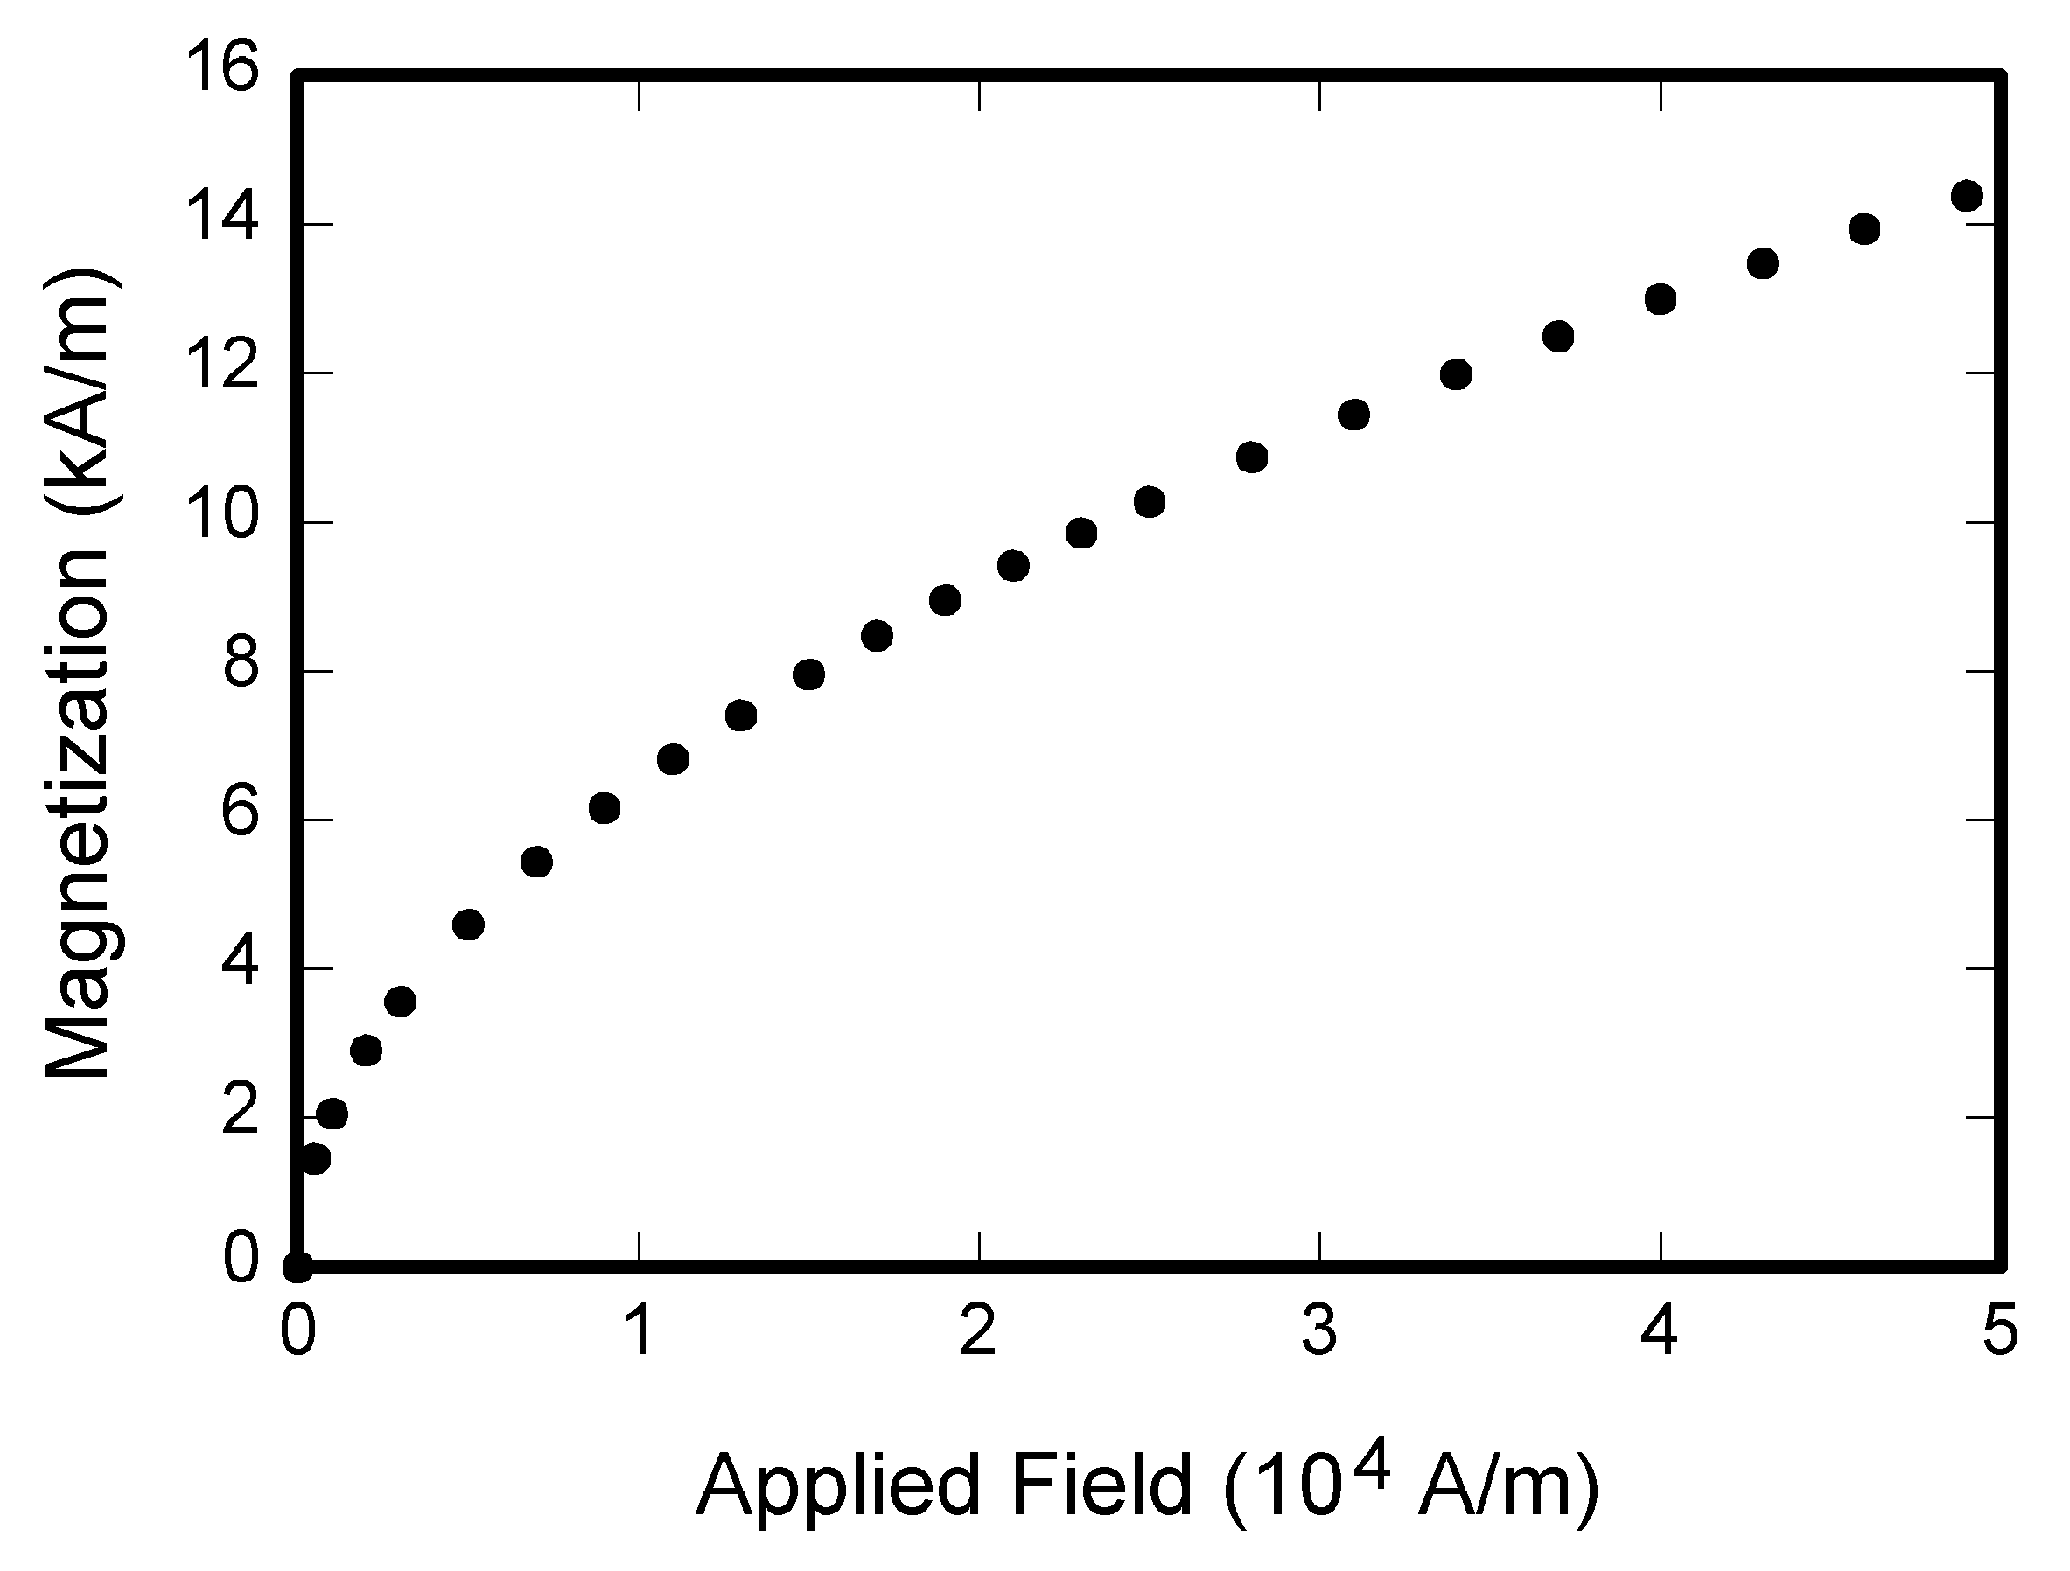
\includegraphics[width=\columnwidth]{fig1.png}}
\caption{Magnetization as a function of applied field. Note that ``Fig.'' is abbreviated. There is a period after the figure number, followed by two spaces. It is good practice to explain the significance of the figure in the caption.}
\end{figure}


\section{Conclusion}

A conclusion section is not required. Although a conclusion may review the main points of the paper, do not replicate the abstract as the conclusion. A conclusion might elaborate on the importance of the work or suggest applications and extensions. 

\section*{Acknowledgment}

The preferred spelling of the word ``acknowledgment'' in American English is without an ``e'' after the ``g.'' Use the singular heading even if you have many acknowledgments. Avoid expressions such as ``One of us (S.B.A.) would like to thank . . . .'' Instead, write “F. A. Author thanks ... .” In most cases, sponsor and financial support acknowledgments are placed in the unnumbered footnote on the first page, not here.

\section*{References and Footnotes}

\subsection{References}

References need not be cited in text. When they are, they appear on the line, in square brackets, inside the punctuation.  Multiple references are each numbered with separate brackets. When citing a section in a book, please give the relevant page numbers. In text, refer simply to the reference number. Do not use ``Ref.'' or ``reference'' except at the beginning of a sentence: ``Reference [3] shows . . . .'' Please do not use automatic endnotes in {\em Word}, rather, type the reference list at the end of the paper using the ``References'' style.

Reference numbers are set flush left and form a column of their own, hanging out beyond the body of the reference. The reference numbers are on the line, enclosed in square brackets. In all references, the given name of the author or editor is abbreviated to the initial only and precedes the last name. Use them all; use {\em et al.} only if names are not given. Use commas around Jr., Sr., and III in names. Abbreviate conference titles.  When citing IEEE transactions, provide the issue number, page range, volume number, year, and/or month if available. When referencing a patent, provide the day and the month of issue, or application. References may not include all information; please obtain and include relevant information. Do not combine references. There must be only one reference with each number. If there is a URL included with the print reference, it can be included at the end of the reference.

Other than books, capitalize only the first word in a paper title, except for proper nouns and element symbols. For papers published in translation journals, please give the English citation first, followed by the original foreign-language citation. See the end of this document for formats and examples of common references. For a complete discussion of references and their formats, see the IEEE style manual at www.ieee.org/authortools.

\subsection{Footnotes}

Number footnotes separately in superscripts (Insert $\mid$ Footnote).\footnote{It is recommended that footnotes be avoided (except for the unnumbered footnote with the receipt date on the first page). Instead, try to integrate the footnote information into the text.}  Place the actual footnote at the bottom of the column in which it is cited; do not put footnotes in the reference list (endnotes). Use letters for table footnotes (see Table I). 


\section*{References}

\subsection*{Basic format for books:}

J. K. Author, ``Title of chapter in the book,'' in {\em Title of His Published Book}, xth ed. City of Publisher, (only U.S. State), Country: Abbrev. of Publisher, year, ch. x, sec. x, pp. xxx--xxx.

\subsection*{Examples:}
\def\refname{}
\begin{thebibliography}{34}

\bibitem{}G. O. Young, ``Synthetic structure of industrial plastics,'' in {\em Plastics}, 2nd ed., vol. 3, J. Peters, Ed. New York, NY, USA: McGraw-Hill, 1964, pp. 15--64.

\bibitem{}W.-K. Chen, {\it Linear Networks and Systems}. Belmont, CA, USA: Wadsworth, 1993, pp. 123--135.

\end{thebibliography}

\subsection*{Basic format for periodicals:}

J. K. Author, ``Name of paper,'' Abbrev. Title of Periodical, vol. x,   no. x, pp. xxx--xxx, Abbrev. Month, year, DOI. 10.1109.XXX.123--456.

\subsection*{Examples:}

\begin{thebibliography}{34}
\setcounter{enumiv}{2}

\bibitem{}J. U. Duncombe, ``Infrared navigation Part I: An assessment of feasibility,'' {\em IEEE Trans. Electron Devices}, vol. ED-11, no. 1, pp. 34--39, Jan. 1959,10.1109/TED.2016.2628402.

\bibitem{}E. P. Wigner, ``Theory of traveling-wave optical laser,''
{\em Phys. Rev.},  vol. 134, pp. A635--A646, Dec. 1965.

\bibitem{}E. H. Miller, ``A note on reflector arrays,'' {\em IEEE Trans. Antennas Propagat.}, to be published.
\end{thebibliography}


\subsection*{Basic format for reports:}

J. K. Author, ``Title of report,'' Abbrev. Name of Co., City of Co., Abbrev. State, Country, Rep. xxx, year.

\subsection*{Examples:}
\begin{thebibliography}{34}
\setcounter{enumiv}{5}

\bibitem{} E. E. Reber, R. L. Michell, and C. J. Carter, ``Oxygen absorption in the earth’s atmosphere,'' Aerospace Corp., Los Angeles, CA, USA, Tech. Rep. TR-0200 (4230-46)-3, Nov. 1988.

\bibitem{} J. H. Davis and J. R. Cogdell, ``Calibration program for the 16-foot antenna,'' Elect. Eng. Res. Lab., Univ. Texas, Austin, TX, USA, Tech. Memo. NGL-006-69-3, Nov. 15, 1987.
\end{thebibliography}

\subsection*{Basic format for handbooks:}

{\em Name of Manual/Handbook}, x ed., Abbrev. Name of Co., City of Co., Abbrev. State, Country, year, pp. xxx--xxx.

\subsection*{Examples:}

\begin{thebibliography}{34}
\setcounter{enumiv}{7}

\bibitem{} {\em Transmission Systems for Communications}, 3rd ed., Western Electric Co., Winston-Salem, NC, USA, 1985, pp. 44--60.

\bibitem{} {\em Motorola Semiconductor Data Manual}, Motorola Semiconductor Products Inc., Phoenix, AZ, USA, 1989.
\end{thebibliography}

\subsection*{Basic format for books (when available online):}

J. K. Author, ``Title of chapter in the book,'' in {\em Title of Published Book}, xth ed. City of Publisher, State, Country: Abbrev. of Publisher, year, ch. x, sec. x, pp. xxx xxx. [Online]. Available: http://www.web.com 

\subsection*{Examples:}

\begin{thebibliography}{34}
\setcounter{enumiv}{9}

\bibitem{}G. O. Young, ``Synthetic structure of industrial plastics,'' in Plastics, vol. 3, Polymers of Hexadromicon, J. Peters, Ed., 2nd ed. New York, NY, USA: McGraw-Hill, 1964, pp. 15--64. [Online]. Available: http://www.bookref.com. 

\bibitem{} {\em The Founders Constitution}, Philip B. Kurland and Ralph Lerner, eds., Chicago, IL, USA: Univ. Chicago Press, 1987. [Online]. Available: http://press-pubs.uchicago.edu/founders/

\bibitem{} The Terahertz Wave eBook. ZOmega Terahertz Corp., 2014. [Online]. Available: http://dl.z-thz.com/eBook/zomega\_ebook\_pdf\_1206\_sr.pdf. Accessed on: May 19, 2014. 

\bibitem{} Philip B. Kurland and Ralph Lerner, eds., {\em The Founders Constitution}. Chicago, IL, USA: Univ. of Chicago Press, 1987, Accessed on: Feb. 28, 2010, [Online] Available: http://press-pubs.uchicago.edu/founders/ 
\end{thebibliography}

\subsection*{Basic format for journals (when available online):}

J. K. Author, ``Name of paper,'' {\em Abbrev. Title of Periodical}, vol. x, no. x, pp. xxx--xxx, Abbrev. Month, year. Accessed on: Month, Day, year, doi: 10.1109.XXX.123456, [Online].

\subsection*{Examples:}

\begin{thebibliography}{34}
\setcounter{enumiv}{13}

\bibitem{}J. S. Turner, ``New directions in communications,'' {\em IEEE J. Sel. Areas Commun.}, vol. 13, no. 1, pp. 11--23, Jan. 1995. 

\bibitem{} W. P. Risk, G. S. Kino, and H. J. Shaw, ``Fiber-optic frequency shifter using a surface acoustic wave incident at an oblique angle,'' {\em Opt. Lett.}, vol. 11, no. 2, pp. 115--117, Feb. 1986.

\bibitem{} P. Kopyt {\em et al.}, ``Electric properties of graphene-based conductive layers from DC up to terahertz range,'' {\em IEEE THz Sci. Technol.}, to be published. doi: 10.1109/TTHZ.2016.2544142.
\end{thebibliography}

\subsection*{Basic format for papers presented at conferences (when available online):}

J.K. Author. (year, month). Title. presented at abbrev. conference title. [Type of Medium]. Available: site/path/file

\subsection*{Example:}

\begin{thebibliography}{34}
\setcounter{enumiv}{16}

\bibitem{}PROCESS Corporation, Boston, MA, USA. Intranets: Internet technologies deployed behind the firewall for corporate productivity. Presented at INET96 Annual Meeting. [Online]. Available: http://home.process.com/Intranets/wp2.htp
\end{thebibliography}

\subsection*{Basic format for reports  and  handbooks (when available online):}
  
J. K. Author. ``Title of report,'' Company. City, State, Country. Rep. no., (optional: vol./issue), Date. [Online] Available: site/path/file 

\subsection*{Examples:}

\begin{thebibliography}{34}
\setcounter{enumiv}{17}

\bibitem{}R. J. Hijmans and J. van Etten, ``Raster: Geographic analysis and modeling with raster data,'' R Package Version 2.0-12, Jan. 12, 2012. [Online]. Available: http://CRAN.R-project.org/package=raster 

\bibitem{}Teralyzer. Lytera UG, Kirchhain, Germany [Online]. Available: http://www.lytera.de/Terahertz\_THz\_Spectroscopy.php?id=home, Accessed on: Jun. 5, 2014.
\end{thebibliography}

\subsection*{Basic format for computer programs and electronic documents (when available online):}

Legislative body. Number of Congress, Session. (year, month day). {\em Number of bill or resolution, Title}. [Type of medium]. Available: site/path/file
{\em NOTE:} ISO recommends that capitalization follow the accepted practice for the language or script in which the information is given.

\subsection*{Example:}

\begin{thebibliography}{34}
\setcounter{enumiv}{19}

\bibitem{}U. S. House. 102nd Congress, 1st Session. (1991, Jan. 11). {\em H. Con. Res. 1, Sense of the Congress on Approval of Military Action}. [Online]. Available: LEXIS Library: GENFED File: BILLS 
\end{thebibliography}

\subsection*{Basic format for patents (when available online):}

Name of the invention, by inventor’s name. (year, month day). Patent Number [Type of medium]. Available:site/path/file

\subsection*{Example:}

\begin{thebibliography}{34}
\setcounter{enumiv}{20}

\bibitem{}Musical tooth brush with mirror, by L. M. R. Brooks. (1992, May 19). Patent D 326 189
[Online]. Available: NEXIS Library: LEXPAT File:   DES 

\end{thebibliography}

\subsection*{Basic format for conference proceedings (published):}

J. K. Author, ``Title of paper,'' in {\em Abbreviated Name of Conf.}, City of Conf., Abbrev. State (if given), Country, year, pp. xxx--xxx.

\subsection*{Example:}

\begin{thebibliography}{34}
\setcounter{enumiv}{21}

\bibitem{}D. B. Payne and J. R. Stern, ``Wavelength-switched passively coupled single-mode optical network,'' in {\em Proc. IOOC-ECOC}, Boston, MA, USA, 1985,
pp. 585--590.

\end{thebibliography}

\subsection*{Example for papers presented at conferences (unpublished):}

\begin{thebibliography}{34}
\setcounter{enumiv}{22}

\bibitem{}D. E behard and E. Voges, ``Digital single sideband detection for inter ferometric sensors,'' presented at the {\em 2nd Int. Conf. Optical Fiber Sensors}, Stuttgart, Germany, Jan. 2--5, 1984.
\end{thebibliography}

\subsection*{Basic formatfor patents:}

J. K. Author, ``Title of patent,'' U. S. Patent x xxx xxx, Abbrev. Month, day, year.

\subsection*{Example:}

\begin{thebibliography}{34}
\setcounter{enumiv}{23}

\bibitem{}G. Brandli and M. Dick, ``Alternating current fed power supply,'' U. S. Patent 4 084 217, Nov. 4, 1978.
\end{thebibliography}

\subsection*{Basic format for theses (M.S.) and dissertations (Ph.D.):}

a) J. K. Author, ``Title of thesis,'' M. S. thesis, Abbrev. Dept., Abbrev. Univ., City of Univ., Abbrev. State, year.

b) J. K. Author, ``Title of dissertation,'' Ph.D. dissertation, Abbrev. Dept., Abbrev. Univ., City of Univ., Abbrev. State, year.

\subsection*{Examples:}

\begin{thebibliography}{34}
\setcounter{enumiv}{24}

\bibitem{}J. O. Williams, ``Narrow-band analyzer,'' Ph.D. dissertation, Dept. Elect. Eng., Harvard Univ., Cambridge, MA, USA, 1993.

\bibitem{}N. Kawasaki, ``Parametric study of thermal and chemical nonequilibrium nozzle flow,'' M.S. thesis, Dept. Electron. Eng., Osaka Univ., Osaka, Japan, 1993.
\end{thebibliography}

\subsection*{Basic format for the most common types of unpublished references:}

a) J. K. Author, private communication, Abbrev. Month, year.

b) J. K. Author, ``Title of paper,'' unpublished.

c) J. K. Author, ``Title of paper,'' to be published.

\subsection*{Examples:}

\begin{thebibliography}{34}
\setcounter{enumiv}{26}

\bibitem{}A. Harrison, private communication, May 1995.

\bibitem{}B. Smith, ``An approach to graphs of linear forms,'' unpublished.

\bibitem{}A. Brahms, ``Representation error for real numbers in binary computer arithmetic,'' IEEE Computer Group Repository, Paper R-67-85.
\end{thebibliography}

\subsection*{Basic formats for standards:}

a) {\em Title of Standard}, Standard number, date.

b) {\em Title of Standard}, Standard number, Corporate author, location, date.

\subsection*{Examples:}

\begin{thebibliography}{34}
\setcounter{enumiv}{29}


\bibitem{}IEEE Criteria for Class IE Electric Systems, IEEE Standard 308, 1969.

\bibitem{} Letter Symbols for Quantities, ANSI Standard Y10.5-1968.
\end{thebibliography}

\subsection*{Article number in reference examples:}

\begin{thebibliography}{34}
\setcounter{enumiv}{31}

\bibitem{}R. Fardel, M. Nagel, F. Nuesch, T. Lippert, and A. Wokaun, ``Fabrication of organic light emitting diode pixels by laser-assisted forward transfer,'' {\em Appl. Phys. Lett.}, vol. 91, no. 6, Aug. 2007, Art. no. 061103. 

\bibitem{} J. Zhang and N. Tansu, ``Optical gain and laser characteristics of InGaN quantum wells on ternary InGaN substrates,'' {\em IEEE Photon.} J., vol. 5, no. 2, Apr. 2013, Art. no. 2600111
\end{thebibliography}

\subsection*{Example when using et al.:}

\begin{thebibliography}{34}
\setcounter{enumiv}{33}

\bibitem{}S. Azodolmolky {\em et al.}, Experimental demonstration of an impairment aware network planning and operation tool for transparent/translucent optical networks,'' {\em J. Lightw. Technol.}, vol. 29, no. 4, pp. 439--448, Sep. 2011.
\end{thebibliography}

\end{document}
